\documentclass[10pt,a4paper]{article}
\usepackage[latin1]{inputenc}
\usepackage[dutch]{babel}
\usepackage{amsmath}
\usepackage{amsfonts}
\usepackage{amssymb}
\usepackage{graphicx}
\usepackage{listings}
\author{Ruben Van Assche}
\title{Wetenschappelijk Programmeren: Oefening 2}
\begin{document}
\maketitle
\section{Opgave}
In deze opgave moest uit een tabel gegeven data een polynomische interpolatie en natuurlijke en kubische spline gehaald worden. Deze moest dan geplot worden om vervolgens de beste interpolatie te selecteren.
\section{Omzetting Data}
De originele x-as inde tabel werd voorgesteld door data(dd/mm/jjjj), dit is niet de beste manier om onze x-as voor te stellen. We verkiezen hier een x-as die start bij 0 en elke datum hier op plot door het aantal dagen tussen data te tellen. Wanneer we deze berkening maken bekomen we volgende tabel:
\newline

\begin{tabular}{lccr}
\textbf{Datum} & \textbf{Gewicht Baby} & \textbf{\# Dagen tussen vorige datum} & \textbf{Nieuwe x-waarde} \\
27/10/2001     & 2.8                   & 0                                     & 0                        \\
19/11/2001     & 3.6                   & 23                                    & 23                       \\
03/12/2001     & 4.4                   & 14                                    & 37                       \\
20/12/2001     & 5.5                   & 17                                    & 54                       \\
09/01/2002     & 6.4                   & 20                                    & 74                       \\
23/01/2002     & 7.2                   & 14                                    & 88                       \\
06/03/2002     & 8.3                   & 42                                    & 130                     
\end{tabular}

\section{Plotten}
Voor het plotten van elke interpolant wordt deze eerst berekend, vervolgens wordt er op het interval $\left [ 0, 130 \right ]$ telkens met een stap van 0.1 een evaluatie van de interpolant gedaan, de behorende y waarde en de x waarde worden vervolgens opgeslagen in een bestand. Dit bestand wordt dan geplot d.m.v. GNUPlot.
\newline
\newline
In de volgende secties overloop ik elke interpolatie methode en probeer te bespreken waarom de bepaalde methode dan wel of niet goed is voor deze set datapunten.

\section{Polynomische Spline}
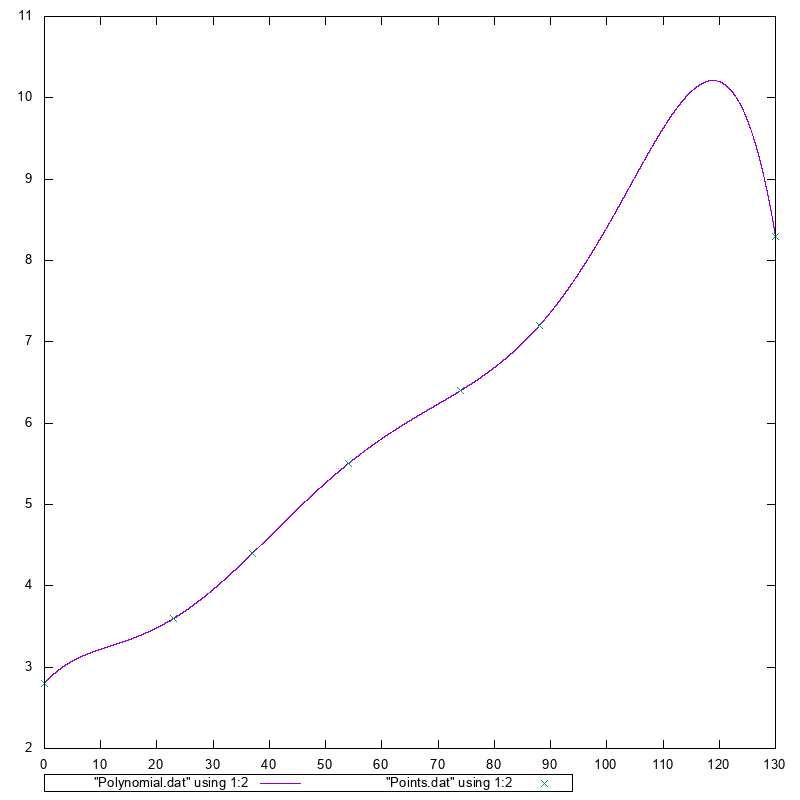
\includegraphics[scale=0.7]{Polynomial}
Het eerste wat bij de polynomische interpolant opvalt is dat deze niet geschikt is om de dataset te interpoleren. Het Runghe fenomeen treed hier duidelijk op, doordat er te veel datapunten voor de interpolant zijn(7) begint de polynomische interpolant te oscilleren. Dit zien we duidelijk op het einde van de functie $\left [ 90, 130 \right ]$ waar de functie een oscillatie maakt inplaats van mooi door te lopen.

\section{Kubische Spline}
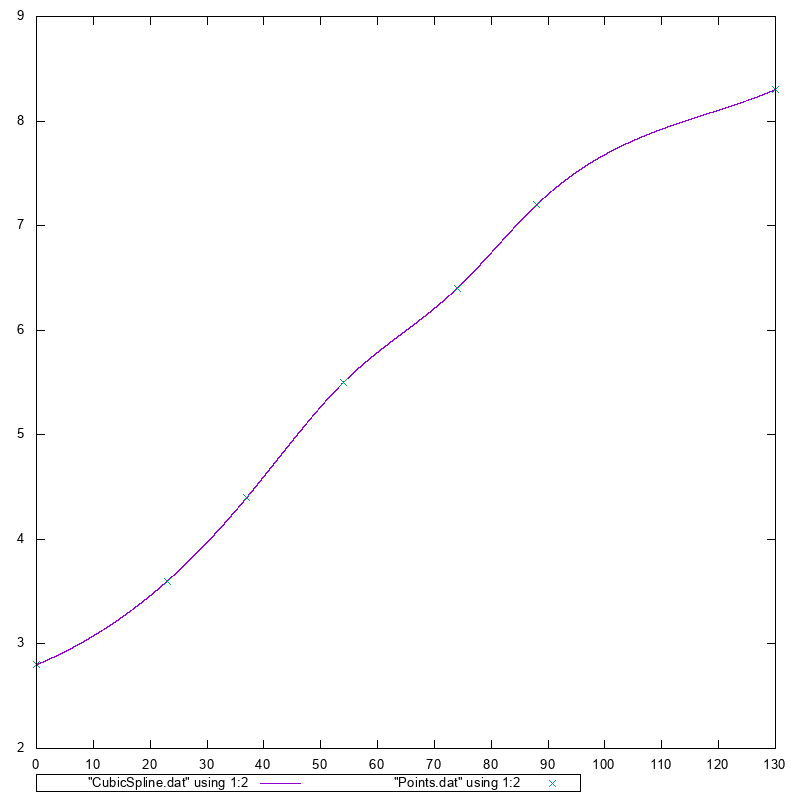
\includegraphics[scale=0.7]{CubicSpline}
Deze interpolatie ziet er al veel beter uit dan de Polynomische interpolatie. De kubische spline loopt veel vloeiender door en lijkt de perfectie te benaderen. Maar we zien toch nog een paar foutjes op het einde $\left [ 90, 130 \right ]$ waar de functie toch wat minder concaaf is als verwacht. Dit komt omdat GSL bij de kubische spline een gelijke y waarde voor begin en eindpunt vraagt anders treden er kleine foutjes zoals deze op.

\section{Natuurlijke Spline}
\includegraphics[scale=0.7]{NaturalSpline}
Om onze data te plotten maken we gebruik van de natuurlijk spline, deze heeft een mooi vloeiend verloop over de gehele functie dit omdat de tweede afgeleide van het begin en eindpunt 0 is.

\section{Conclusie}
Waar de polynomische functie faalt om de data te interpoleren, slaagt de kubische spline er zeker al in om een mooi resultaat te laten zien alhoewel ik toch de natuurlijke spline verkies welke net iets mooier loopt.

\section{Code}
\textbf{Main.cpp - De code voor het berekenen van de punten door de interpolant}
\lstinputlisting{../main.cpp}

\textbf{graphs.gnuplot - De code voor tekenen berekenen van de interpolant}
\lstinputlisting{../graphs.gnuplot}

\end{document}